%% --------------------------------------------------------------------------
% LaTeX template for the XLIV CILAMCE
%
% This latex document tries to copy the Microsoft Word template.
% --------------------------------------------------------------------------
\documentclass[a4paper,10pt]{book}

% PACKAGES USED - packages that need to be previously installed on your computer
\usepackage[lmargin=2.5cm, rmargin=2.5cm, tmargin=2.5cm, bmargin=2.5cm ]{geometry}
\usepackage{graphicx}
\usepackage{times}
\usepackage{indentfirst}
\usepackage{fancyhdr}
\usepackage{titlesec}
\usepackage[english]{babel}
\usepackage{parskip} 
\usepackage{setspace}

%Package to hold figure in position
\usepackage{placeins}


% Mathematical Symbols
\newcommand{\dgds}{\boldsymbol{g_\sigma}}
\newcommand{\Dll}{\boldsymbol{D}}
\newcommand{\Dllmod}{\boldsymbol{D^{*}}}
\newcommand{\Dllepvp}{\boldsymbol{D}^{epvp}}
\newcommand{\dstrain}{\boldsymbol{\dot{\varepsilon}}}
\newcommand{\dstraine}{\boldsymbol{\dot{\varepsilon}}^{e}}
\newcommand{\dstrainp}{\boldsymbol{\dot{\varepsilon}}^{p}}
\newcommand{\dstrainv}{\boldsymbol{\dot{\varepsilon}}^{vp}}
\newcommand{\straineqp}{\bar \varepsilon^p}
\newcommand{\dstrainsh}{\boldsymbol{\dot{\varepsilon}}^{sh}}
\newcommand{\dstraincr}{\boldsymbol{\dot{\varepsilon}}^{cr}}
\newcommand{\dstress}{\boldsymbol{\dot{\sigma}}}

\newcommand{\ex}{\boldsymbol{e}_x}
\newcommand{\ey}{\boldsymbol{e}_y}
\newcommand{\ez}{\boldsymbol{e}_z}

\newcommand{\onell}{\boldsymbol{1}}
\newcommand{\strain}{\boldsymbol{\varepsilon}}
\newcommand{\straincr}{\boldsymbol{\varepsilon}^{cr}}
\newcommand{\straine}{\boldsymbol{\varepsilon}^{e}}
\newcommand{\strainp}{\boldsymbol{\varepsilon}^{p}}
\newcommand{\strainsh}{\boldsymbol{\varepsilon}^{sh}}
\newcommand{\strainshCEB}{\varepsilon_{sh}}
\newcommand{\strainvp}{\boldsymbol{\varepsilon}^{vp}}
\newcommand{\stress}{\boldsymbol{\sigma}}
\newcommand{\zerol}{\boldsymbol 0}

%%%%%%%%%%%%%%%%%%%%%%%%%%%%%%%%%%%%%%%%%%%%%%%%%%%%%%%%%%%%%%%%%
%%%%%%%%%%%%%%%%%%%%%%%%%%%%%%%%%%%%%%%%%%%%%%%%%%%%%%%%%%%%%%%%%
%%% My Additional Packages
%%%%%%%%%%%%%%%%%%%%%%%%%%%%%%%%%%%%%%%%%%%%%%%%%%%%%%%%%%%%%%%%%
\usepackage[utf8]{inputenc}
\usepackage{amssymb} %Mathematics
\usepackage{amsfonts}%Mathematics
\usepackage{amsmath,amscd}%Mathematics
\usepackage{amsthm}%Mathematics
\usepackage{mathrsfs}%Mathematics font
\usepackage{xspace}
\usepackage{booktabs}
\usepackage{stmaryrd}%Particular Brackets
\usepackage{graphicx} %Tables and Figures
\usepackage{subfigure}
\usepackage{url}
\usepackage{hyperref}
\usepackage{cleveref}
\usepackage{./pkg-crefNames}
\usepackage[labelsep=period]{caption}
%\usepackage{mathptmx}
\usepackage{newtxtext,newtxmath}
\usepackage{bm}




%BibTeX compatible with the CILAMCE format
\usepackage[numbers,sort&compress]{natbib}

\setlength{\bibsep}{0pt plus 0.3ex}

\renewcommand*{\bibfont}{\small}

\makeatletter
\renewcommand\bibsection
{
  \section*{References}
}



\renewenvironment{thebibliography}[1]
      {\section*{\refname}%
       \@mkboth{\MakeUppercase\refname}{\MakeUppercase\refname}%
       \list{\@biblabel{\@arabic\c@enumiv}}%
            {\settowidth\labelwidth{\@biblabel{#1}}%
             \leftmargin\labelwidth
             \advance\leftmargin-10pt% change 20 pt according to your needs
             \advance\leftmargin\labelsep
             \setlength\itemindent{10pt}% change using the inverse of the length used before
             \@openbib@code
             \usecounter{enumiv}%
             \let\p@enumiv\@empty
             \renewcommand\theenumiv{\@arabic\c@enumiv}}%
       \sloppy
       \clubpenalty4000
       \@clubpenalty \clubpenalty
       \widowpenalty4000%
       \sfcode`\.\@m}
      {\def\@noitemerr
        {\@latex@warning{Empty `thebibliography' environment}}%
       \endlist}
\renewcommand\newblock{\hskip .11em\@plus.33em\@minus.07em}
\makeatother




\makeatother
\bibliographystyle{./bib-cilamce}
%\bibliographystyle{plain}


%%%%%%%%%%%%%%%%%%%%%%%%%%%%%%%%%%%%%%%%%%%%%%%%%%%%%%%%%%%%%%%%%
%%%%%%%%%%%%%%%%%%%%%%%%%%%%%%%%%%%%%%%%%%%%%%%%%%%%%%%%%%%%%%%%%

% CONFIGURATION
\renewcommand*\arraystretch{1.5}
\renewcommand*\thesection{\arabic{section}}
%\hyphenpenalty=10000 % You can uncomment this to avoid hyphenization
\titleformat*{\section}{\large\bfseries}
\titleformat*{\subsection}{\bfseries}
\titlespacing\section{0pt}{20pt plus 2pt minus 2pt}{12pt plus 2pt minus 2pt}
\titlespacing\subsection{0pt}{20pt plus 0pt minus 0pt}{12pt plus 0pt minus 0pt}
\setlength{\parskip}{0pt} % Spacing between paragraphs
\setlength{\parindent}{0.75cm} % Paragraph identation
\setlength\abovecaptionskip{6pt}

% --------------------------------------------------------------------------
% DO NOT EDIT - SPECIAL HEADINGS OF XLIII CILAMCE
% --------------------------------------------------------------------------
\fancypagestyle{first}
{
\fancyhf{}
\fancyfoot[RO]{\footnotesize \textit{CILAMCE-2024 \\
Proceedings of the XLV Ibero-Latin-American Congress on Computational Methods in Engineering, ABMEC\\
Maceió, Alagoas, November 11-14, 2024}}
\renewcommand{\headrulewidth}{.0pt}
\renewcommand{\footrulewidth}{.5pt}
}

\pagestyle{fancy}
\fancyhf{}

\fancyfoot[LE]{\footnotesize \textit{CILAMCE-2024\\
Proceedings of the XLV Ibero-Latin-American Congress on Computational Methods in Engineering, ABMEC\\
Maceió, Alagoas, November 11-14, 2024}}

\fancyfoot[RO]{\footnotesize \textit{CILAMCE-2024\\
Proceedings of the XLV Ibero-Latin-American Congress on Computational Methods in Engineering, ABMEC\\
Maceió, Alagoas, November 11-14, 2024}}




\renewcommand{\headrulewidth}{.5pt}
\renewcommand{\footrulewidth}{.5pt}

% --------------------------------------------------------------------------
% PLEASE, EDIT THIS!
\fancyhead[LE]{\footnotesize \textit{Finite Element Analysis of Rock Deformation in Deep Twin Tunnels}}
\fancyhead[RO]{\footnotesize \textit{Felipe P. M. Quevedo, Carlos A. M. M. Colombo, Bianca M. Girardi, Denise Bernaud, Samir Maghous}}
% --------------------------------------------------------------------------

\begin{document}\thispagestyle{first}

% --------------------------------------------------------------------------
% DO NOT EDIT - LOGO OF XLIII CILAMCE
% --------------------------------------------------------------------------

\begin{figure}[ht!]
\vspace{-30pt}
\flushright

\includegraphics[width=4.3cm]{Figures/logo.png}
%scale=0.25
\end{figure}

% --------------------------------------------------------------------------
% TITLE OF PAPER
% --------------------------------------------------------------------------

\noindent
\textbf{\Large
Finite Element Analysis of Rock Deformation in Deep Twin Tunnels} 
\vspace{18pt} % <- keep this vertical space!

% --------------------------------------------------------------------------
% AUTHORS
% --------------------------------------------------------------------------

\noindent Felipe P. M. Quevedo$^1$, Carlos A. M. M. Colombo$^1$, Bianca M. Girardi$^1$, Denise Bernaud$^1$, Samir Maghous$^1$

\vspace{18pt} % <- keep this vertical space!

\noindent $^1$\textit{Federal University of Rio Grande do Sul}

\noindent \textit{Av. Osvaldo Aranha, 99, Porto Alegre, 90.035-190, RS, Brazil}

\noindent \textit{motta.quevedo@ufrgs.br, ca-colombo@hotmail.com, eng.biancagirardi@gmail.com}

\noindent \textit{denise.bernaud@ufrgs.br, samir.maghous@ufrgs.br}


\vspace{18pt} % <- keep this vertical space!

% --------------------------------------------------------------------------
% ABSTRACT
% --------------------------------------------------------------------------

\noindent \textbf{Abstract.}
Relying upon a three-dimensional finite element analysis, this contribution investigates the instantaneous irreversivel response induced by the constitutive behavior of the rock mass in the convergence profile of twin tunnels with gallery. At the rock material level, elastoplastic state equations based on a Drucker-Prager yield surface with an associated flow rule are adopted in the modeling. As regards the tunnel support, the formulation accounts for the presence of an elastic shotcrete-like lining. From a computational point of view, the deactivation-activation method is used to simulate the excavation process and the installation of the lining. The accuracy of the finite element predictions is assessed through comparisons with the available analytical solutions formulated in a simplified scenario for the twin tunnel configuration. A parametric study investigates the mutual interaction induced by the proximity of the tunnels and effects of the stiff of lining.

\vspace{18pt} % <- keep this vertical space!

\noindent \textbf{Keywords:} Twin tunnels, Elastoplasticity, Finite element modeling


% --------------------------------------------------------------------------
\section{Introduction}\label{sec:introduction}
% --------------------------------------------------------------------------
Many design methods often focus on single tunnels, but twin tunnels are a common occurrence. The interaction between tunnels can be significant, especially when the spacing between them is minimal. Additionally, many twin tunnels incorporate transverse galleries, introducing a localized effect on displacements and stresses. While the simulation of tunnel convergence in single tunnels has been widely investigated and reported in published
literature, few works have addressed the computational evaluation of deformation in twin tunnels. Some studies on deep twin tunnels can be found at \citet{Spyridis2015}, \citet{Chen2019}, \citet{MA2020}, \citet{Fortsakis2021}, \citet{chortis2021a}, \citet{chortis2021b}, \citet{GUO2021}, \citet{chortis2023a}, \citet{chortis2023b}. But less attention has been dedicated to assessing the mutual mechanical interaction induced by the excavation of the transverse gallery connecting the twin tunnels.

In this context, the main contributions of this paper can be summarized at both the material and tunnel analysis levels. At the material level, the constitutive state equations of the rock mass are developed using a plasticity framework, which is suitable for clayey rocks. For the mechanical behavior of the concrete lining, the traditional linear elastic model are employed. At the structural analysis level, the deformation of the highly interactive components of the material system (i.e., rock mass and lining) resulting from the excavation of twin tunnels and transverse gallery is simulated using three-dimensional finite element simulations. The excavation and lining placement processes are simulated through the activation/deactivation technique. The constitutive models for the rock mass and the associated numerical integration schemes, are implemented into the UPF/USERMAT customization tool [\citenum{ANSYS:2013b}] of the ANSYS standard software. This three-dimensional finite element analysis is specifically designed to address the interactions induced by the construction process, the proximity of twin tunnels, and the presence of the transverse gallery.

%Only full-length papers that have been orally presented will be published in the congress proceedings. It is extremely important that you prepare your full-length paper in strict accordance with the text formatting of this document, which can be enforced either using the pre-defined styles of this template file or manually setting the specifications described in the next section. After the preparation of your paper, you should generate a PDF file for submission. Only PDF files will be accepted by the online submission system.

% --------------------------------------------------------------------------
\section{Constitutive Models}\label{sec:format}
% --------------------------------------------------------------------------

%The delayed behavior of constitutive materials is crucial in understanding the deformation of tunnel structures in deep clayey rocks (see for instance \citet{rousset1988}, \citet{Nguyen1987} or \citet{GIRAUD1996}). However, during the early stages of tunnel excavation, the rock mass around the tunnel undergoes severe loading and high strain rates, leading to significant instantaneous irreversible strains near the tunnel wall, which can impact the structure's long-term stability. The model formulation is based on earlier works by \citet{Nguyen1987} and \citet{rousset1988}. For brevity, only the main features of this model are summarized here, with detailed descriptions, applications, and validations available in \citet{quevedo2022b}. The finite element implementation of this model in the USERMAT procedure of ANSYS software is detailed in \citet{quevedo2022thesis}.

The constitutive model for the rock mass corresponds to the associated Drucker-Prager elastoplastic model. The local strain rate $\dstrain$ is split into two contributions $\dstrain = \dstraine + \dstrainp$, so that the constitutive relationships relating the Cauchy stress rate $\dstress$ and strain rate components can be written as:
\begin{equation} \label{eq_constitutive_relationship_epvp}
	\dstress = \Dll : \dstraine = \Dll : (\dstrain - \dstrainp).\;
\end{equation}



% The one-dimensional representation of the constitutive behavior is shown in Fig.~\ref{reological_scheme}.
%\begin{figure}[h!]
%	\centering
%	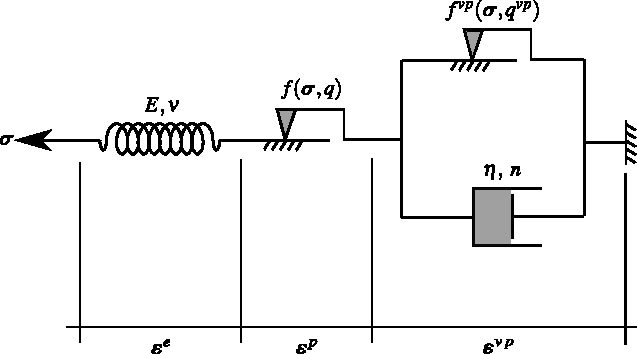
\includegraphics[scale=1]{Figures/Rheological representation.pdf}
%	\caption{Rheological representation of the elastoplastic-viscoplastic model.}
%	\label{reological_scheme}
%\end{figure}

In the above relationship, $\dstraine$ and $\dstrainp$, represent respectively the elastic and plastic strain rate, and $\Dll$ denote the fourth-order isotropic elastic linear constitutive tensor defined by the rock mass elastic Young modulus $E$ and Poisson ratio $\nu$. The plastic strain rate is given by flow rule:
\begin{equation}
	\label{eq_plastic_flow}
	\dot \strainp = \left\{ 
	\begin{array}{ll} 
		\dot \lambda \dfrac{\partial g}{\partial \stress} &  \text{for } f > 0 \\ 
		\zerol, & \text{for } f \le 0 \\
	\end{array}\right.,
\end{equation}
where $\dot \lambda$ is the plasticity multiplier (obtained through the consistency condition  $\dot f = 0$) and $g$ is a potential flow function analogous to $f$ used to simulate the volume dilatation during the evolution of plastic deformations. However, for this analysis, was used associated plasticity, i.e., $g=f$. In this model the Drucker-Prager plastic flow surface is given by
\begin{equation}
	\label{eq:f_Drucker_Prager}
	f(\stress,q) = f(I_1,J_2,q) = \beta_1 I_1 +\beta_2 \sqrt{J_2}-q(\alpha),
\end{equation}
which $I_1$ is the first invariant of the stress tensor, $J_2$ the second invariant of the deviator tensor and $\beta_1, \beta_2$ and $q(\alpha)$ are strength parameters related to the friction angle $\phi$ and cohesion $c(\alpha)$, respectively. In the present model Drucker-Prager surface been inner of the Mohr-Coulomb surface [\citenum{bernaud1991}], that is,
\begin{equation}
	\label{eq:f_DP_inscrita_MC}
	\beta_1 = \dfrac{(k-1)}{3}, ~~~ \beta_2 = \dfrac{(2k+1)}{\sqrt{3}}, ~~~
	q(\alpha) = 2\sqrt{k}~c(\alpha),
\end{equation}
where $k = (1+\sin{\phi})/(1-\sin{\phi})$. The internal variable $\alpha$ is the equivalent plastic strain $\straineqp$ used to simulate strain hardening/softening phenomena. However, for this study, we adopt perfect plasticity, meaning that c is a constant. 

A linear elastic constitutive model is used for the concrete lining, which can be expressed, within the framework of infinitesimal analysis, as $\dstress = \Dll : \dstrain$, where, $\dstraine$ and $\Dll$ are respectively the elastic strain rate and the fourth-order isotrpoic elastic constitutive tensor defined by the concrete lining Poisson ratio $\nu_c$ and elastic Young modulus $E_c$. In the analyses, for comparisons, the tunnel stiffness will be given by the following expression:

\begin{equation} \label{eq:8}
	K_c = \frac{E_c}{1+\nu_c}\frac{R_t^2-(R_t-e_t)^2}{(1-2\nu_c)R_t+(R_t-e_t)^2},
\end{equation}
%\begin{equation} \label{eq:9}
%	E_c = 21500\left[(f_{ck}+8)/10\right]^{1/3}
%\end{equation}
%However, to describe the results, the effect of the lining is best described through its stiffness, given by the following formula:
%\begin{equation} \label{eq:10}
%	K_c = \frac{E_c}{1+\nu_c}\frac{R_t^2-(R_t-e_t)^2}{(1-2\nu_c)R_t^2+(R_t-e)^2}
%\end{equation}
% --------------------------------------------------------------------------
\section{Spatial and time discretization of the domain}\label{sec:format}
% --------------------------------------------------------------------------

The geometry material domain $\Omega$ considered for the finite element simulations is defined by a parallelepiped volume of dimensions $\left(L_1+L_2 \right ) \times L_3 \times d_3$ (\cref{Mesh1}). Owing to the symmetry of the problem, only the material portion $\left\{x \le 0, y \ge 0\right\}$   is considered for F.E discretization and analysis. Referring to the notations of \cref{Mesh1}, $d_1$ is the distance between the axes of longitudinal tunnels, $L_2$  represents the total length  along longitudinal direction $\ez$ of the cylindrical  volume to be excavated that is  considered in the numerical simulation, $d_3$ is the thickness along vertical direction $\ey$ of material domain $\Omega$, $L_1$ stands for the length of unexcavated region after total excavation process, $L_3$ is the total length along transversal direction $\ex$ of discretized material domain, $d_2$ characterizes the location of the circular transverse axis gallery that intersects the  longitudinal tunnel at $z = L_1+d_2$. The length of the excavation step adopted  will be denoted by $L_{pt}$. The mesh used in the simulations consists of $119740$ or $221104$ total elements (hexahedra and tetrahedra), depending on the value of spacing between longitudinal tunnels. To increase the accuracy of the model predictions in the intersection zone, the region surrounding the transverse gallery (including part of the longitudinal tunnel) is discretized by means 10-node quadratic tetrahedral elements, whereas 8-node trilinear hexahedral elements are used for the remaining part of the structure.   Furthermore, a refined meshing is used for discretizing the zones surrounding the longitudinal and transverse gallery. These zones whose mechanical state is significantly affected by the tunnelling process are indicated by light gray color in \cref{Mesh1}. Two values shall be considered for the spacing $d_1$ in the numerical simulations, namely  $d_1 = 16R_t$ and $4R_t$. The layer of concrete lining of thickness $e_g$ installed along the gallery wall is indicated by red color in the figure. Without introducing additional modeling restriction and for the sake of simplicity, the value of the gallery radius is fixed to $R_g = 2/3R_t$. The same lining system (same concrete material and layer thickness) is considered for both longitudinal tunnels and gallery. As regards the discretization of the region surrounding the gallery, parameters $d_5$ and $d_1$ define the size in a $yz$ plane of the transition region involving the tetrahedral finite elements. The initial stress state prevaling in the rock mass prior to the tunnel excavation process is defined by constant vertical and horziontal geostatic stress $\sigma_v$ and $\sigma_h$ taking the following form:
\begin{equation} \label{eq:stress0}
	\stress_0 = -\sigma_v \ey \otimes \ey - \sigma_h\left( \onell - \ey \otimes \ey \right)
\end{equation}

\begin{figure}[h!]
	\centering
	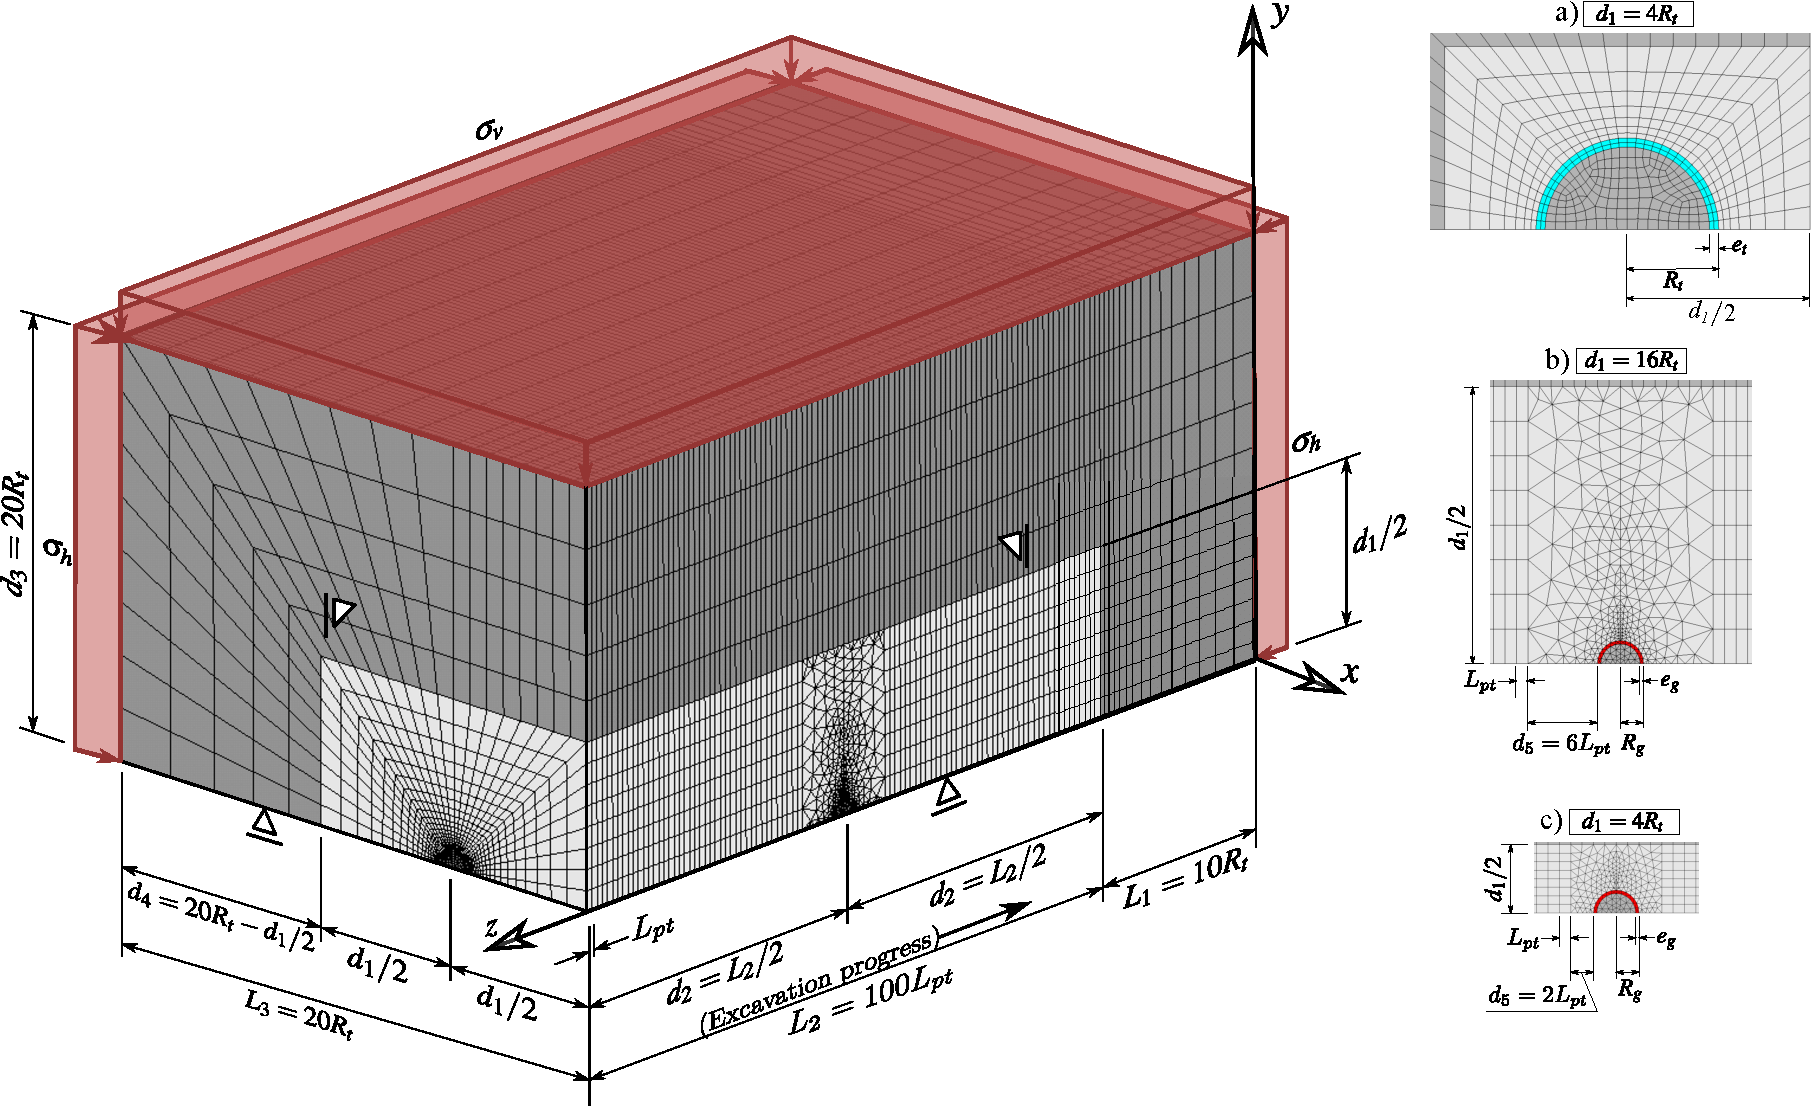
\includegraphics[scale=0.55]{Figures/Mesh1.pdf}
	\caption{Geometry, mesh and boundary conditions of domain and details of a) longitudinal tunnel cross-section for configuration $d_1=4R_t$ and gallery cross-section for configurations b) $d_1=16R_t$ and c) $d_1=4R_t$.}
	\label{Mesh1}
\end{figure}
\FloatBarrier
As mentioned previously, the tunnelling process, including the excavation steps and lining installation, is simulated resorting to the activation-deactivation method shown in the schematic representation in \cref{Diagram of excavations}. Each excavation step is modeled by deactivation of the corresponding elements (the elements stiffness is reduced by a factor $1E8$), whereas installation of elements of lining at a distance $d_{0t}$ from the excavation face (unlined length) is achieved through activation of the corresponding elements by assigning them concrete properties. In this Figure, $n_p$ is the total number of excavation steps and $n_{pig}$ represents the number of longitudinal tunnel excavation steps prior to gallery excavation. After achievement of the $n_{pig}$ excavation steps, the excavation of the gallery is initiated starting from the longitudinal tunnel wall. Referring to the notation of \cref{Diagram of excavations},  $L_{pg}$ is the considered step length for the gallery excavation and $d_{0g}$ is the unlined length of the gallery. After the gallery excavation is completed, we proceed to further excavation steps of the longitudinal tunnel. The main parameters defining the geometry domain as well as and excavation process and lining installation are summarized in Table~\ref{table1}.

\begin{figure}[h!]
	\centering
	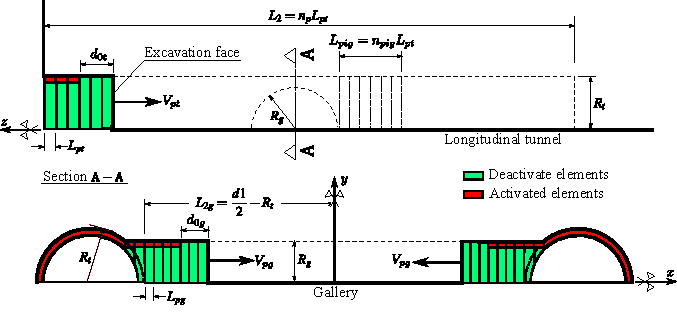
\includegraphics[scale=1.2]{Figures/Diagram of excavations.pdf}
	\caption{Schematic representation of the excavation process.}
	\label{Diagram of excavations}
\end{figure}
\FloatBarrier

\begin{table}
	\caption{Parameters related to the geometry of the domain, excavation and installation of the lining.}
	\label{table1}
	\centering
	%\small
	\renewcommand{\arraystretch}{1.25}
	\begin{tabular}{c c c c}
		\hline
		\multicolumn{1}{c}{PARAMETERS} &
		\multicolumn{1}{c}{SYMBOL} &
		\multicolumn{1}{c}{UNIT} &
		\multicolumn{1}{c}{VALUES} \\
		\hline
		\multicolumn{4}{c}{Longitudinal tunnels} \\
		\hline
		Radius of the longitudinal tunnel & $R_t$ & m & $R_t$ \\
		Thickness of the lining & $e_t$ & m & $0.1R_t$, $0.03R_t$ \\
		Length of the excavation step & $L_{pt}$ & m & $1/3R_t$ \\
		Unlined length & $d_{0t}$ & m & $2L_{pt}$ \\
		\hline
		\multicolumn{4}{c}{Gallery} \\
		\hline
		Radius of the gallery & $R_{g}$ & m & $2/3R_t$ \\
		Thickness of the lining & $e_g$ & m & $e_t$ \\
		Length of the excavation step & $L_{pg}$ & m & $1/3R_g$ \\
		Unlined length & $d_{0g}$ & m & $2L_{pg}$ \\
		Number of steps that starts gallery excavation & $n_{pig}$ & un & $15$ \\
		\hline
		\multicolumn{4}{c}{Rest of domain} \\
		\hline
		Distance between the axes of longitudinal tunnels & $d_1$ & m & $4R_t, ~16R_t$ \\
		Thickness along vertical direction $\ey$ & $d_3$ & m & $20R_t$ \\
		Length of unexcavated region & $L_1$ & m & $10R_t$ \\
		Total excavated length along direction $\ez$ & $L_2$ & m & $100L_{pt}$ \\
		Total length along transversal direction $\ex$ & $L_3$ & m & $20R_t + d_1/2 $ \\
		\hline
	\end{tabular}
	\normalsize
	\\ 
\end{table}
\FloatBarrier
% --------------------------------------------------------------------------
\section{Verification with unlined twin tunnel in elastoplastic medium}\label{sec:format}
% --------------------------------------------------------------------------

In the context of plane strain conditions, Ma et al. [\citenum{MA2020}] developed an approximate analytical solution for the stresses and the plastic zone boundary around deep twin circular tunnels excavated in a homogeneous elastoplastic medium. For the constitutive model, the authors considered perfectly plastic Mohr-Coulomb criterion with associated plastic flow rule. The stress solution for twin tunnels was formulated on the premise that the plastic zone around each tunnel fully encloses the tunnel edge, with the two plastic zones remaining separate and unconnected.

\cref{MA_FIG1} shows the comparison between the 3D F.E. Solution (from a far behind the excavation face) and the analytical solution for plastic zone boundary provided in [\citenum{MA2020}]. For these analysis, $R_t = 1$ m, $d_1/2R_t = 2.5$, rock Young's modulus $E=20$ GPa, Poisson's ratio $\nu = 0.3$ and, friction angle $\phi = 30^\circ$. This analysis shows that finite element modeling produces predictions very similar with those shown in \ref{MA_FIG1}. In addition, the results show that lower values of cohesion $c$ result in larger plastic zones.

\begin{figure}[h!]
	\centering
	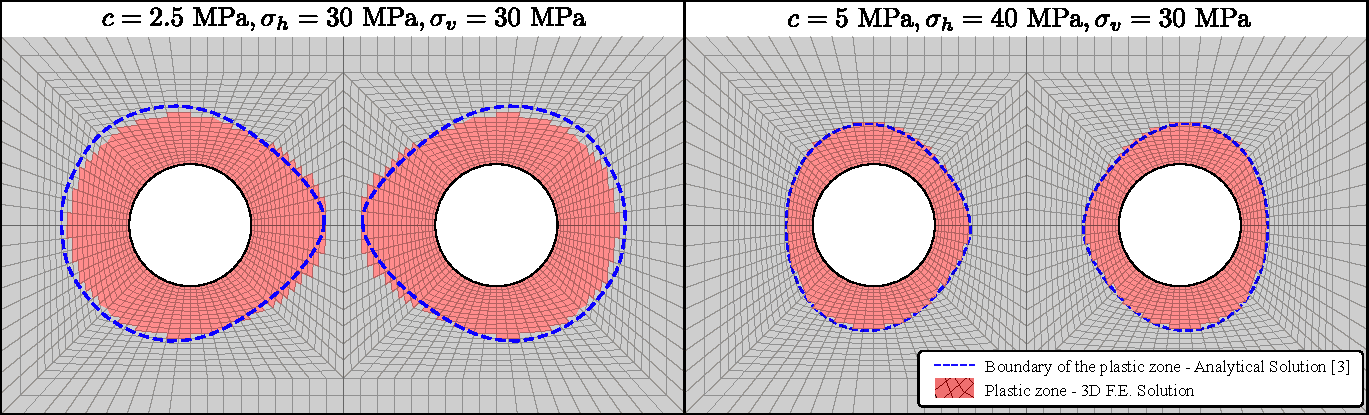
\includegraphics[scale=0.7]{Figures/MA_Comparisions_plastic_zones.pdf}
	\caption{The plastic zone extent obtained from the present F.E. simulations and from the stress solution provided in [\citenum{MA2020}].}
	\label{MA_FIG1}
\end{figure}
\FloatBarrier

Further comparisons are illustrated in Fig.~\ref{MA_stresspaths}, which shows the radial $\sigma_{rr}$ and orthoradial $\sigma_{\theta \theta}$ stress components along three radial paths defined in polar coordinates by $\theta = 45^\circ$, $90^\circ$, and $135^\circ$. It is important to note that although the finite element simulations use the Drucker-Prager yield surface inscribed within the Mohr-Coulomb surface (as used in the solution by Ma et al. \citenum{MA2020}), the numerical predictions closely match the analytical stress solution.

\begin{figure}[h!]
	\centering
	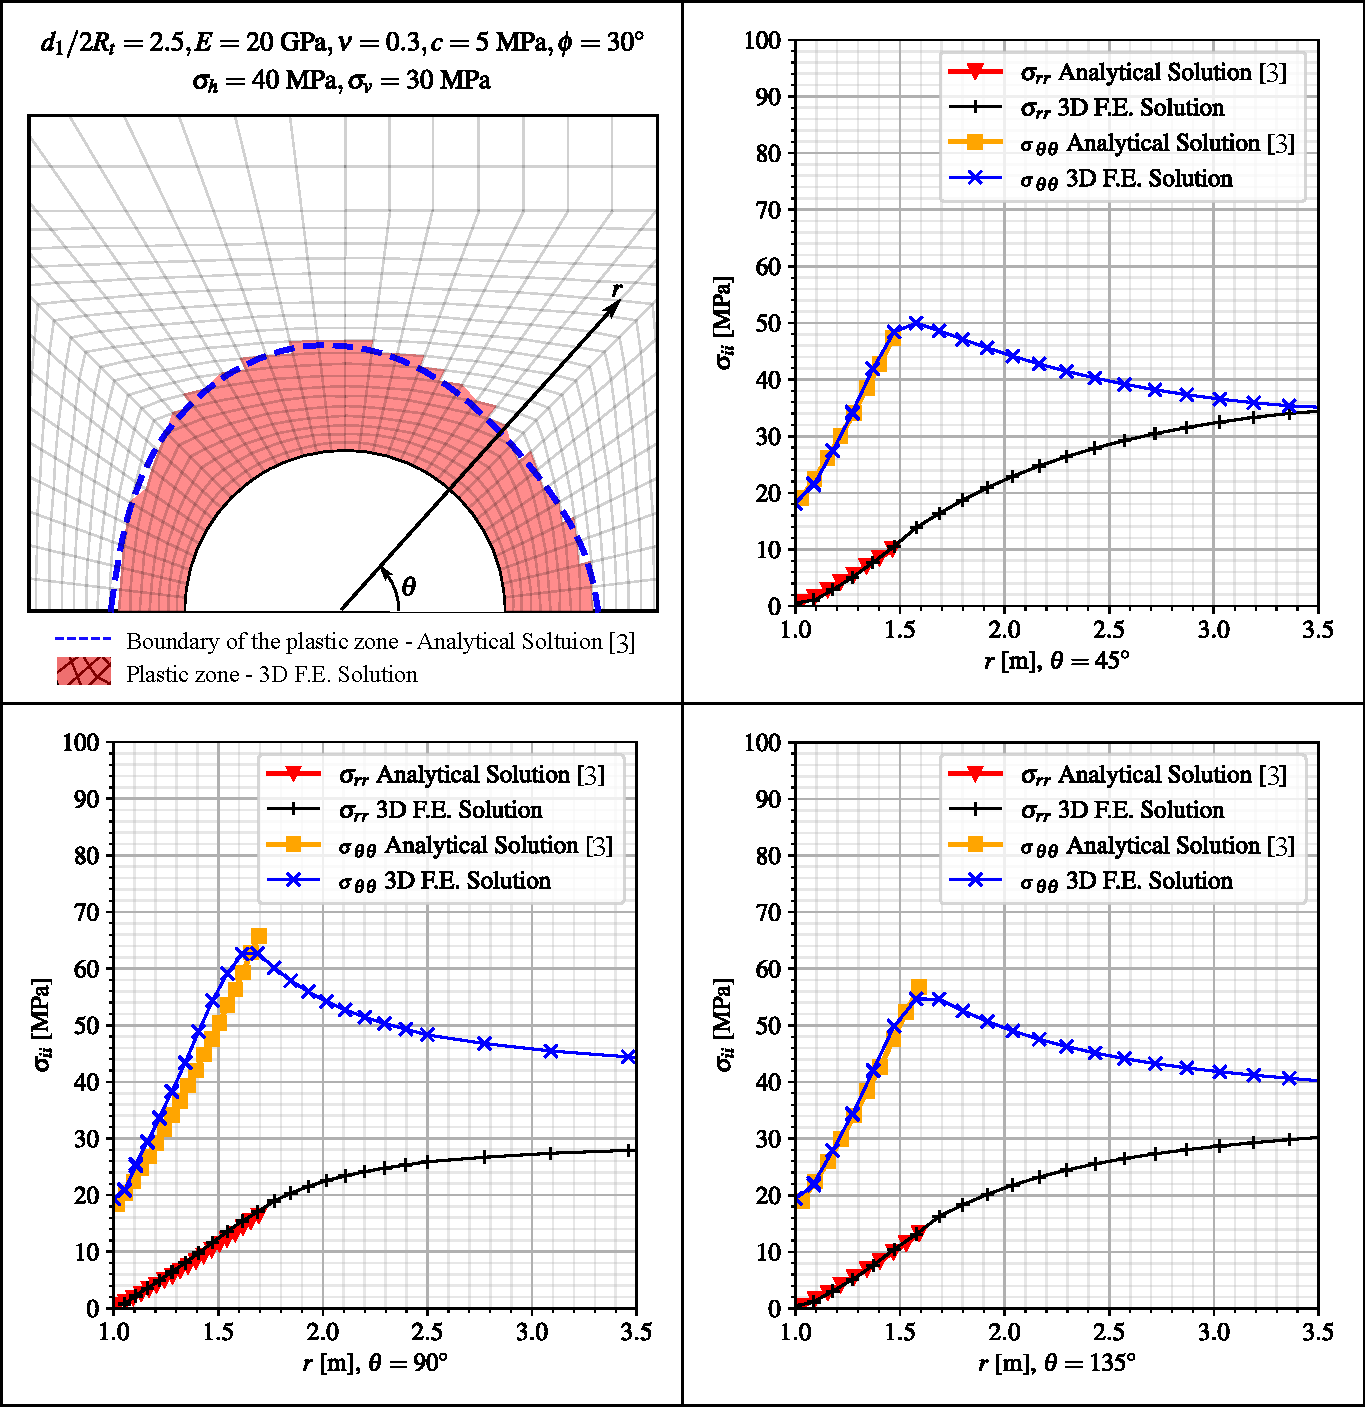
\includegraphics[scale=0.6]{Figures/MA_stresspaths.pdf}
	\caption{Comparisons between the numerical and analytical solution for differents stress-paths.}.
	\label{MA_stresspaths}
\end{figure}
\FloatBarrier

% --------------------------------------------------------------------------
\section{Numerical Results and Discussion}\label{sec:format}
% --------------------------------------------------------------------------
To develop the analysis, we employed Young's modulus $E = 1500$ MPa, Poisson ratio $\nu = 0.49$ (to simulate a incompressible material), $c = 4\sqrt{3}/2$, $\phi = 0^\circ$ and, isotropic initial stresses $\sigma_v = \sigma_h = 9$ MPa, which correspond to the constitutive parameters and tunneling conditions in the clay rock mass in the Paris basin (specifically in Aisne), as detailed in \citet{piepi1995} and \citet{rousset1988}. For the lining, two stiffness values will be considered: $K_c = 969$ MPa and $K_c = 3403$ MPa which assuming a tunnel radius $R_t = 1$ m, $E_c = 30303$ MPa, $\nu_c = 0.2$, these values corresponds to thicknesses $e_t$ of $0.1$ m and $0.03$ m. Denoting by $u_y$ the displacement component following the  $y$-axis, \cref{EP_d1_16Ri} and \cref{EP_d1_4Ri} displays the convergence curves $U_B = -u_y(B)/R_t$ that characterize the inward movement at the tunnel roof $B(x=0,y=R_t,z)$ as a function of normalized longitudinal distance to the facing for different conditions: without lining (NL), with elastic lining (EL), with (WG) and without gallary (NG) for $d_1 = 16R_t$ and $d_1 = 4R_t$, respectively. In these graphs, Uc corresponds to convergence at $z/R_t = -25$ (far from the effect of the excavation face and the gallery).

For the single tunnel, a high stiffness lining (black solid line) decreases convergence by approximately 35\% compared to the unlined model (black dashed line). Conversely, a moderately stiff lining (black dotted line) increases convergence by 12\% compared to the rigid lining.

When $d_1 = 16R_t$ between the twin tunnels (blue and yellow lines), the results of $U_{eq}$ are similar to the isolated tunnel (black line). However, with a distance reduced to $d_1 = 4R_t$, the interaction between the tunnels becomes significant. A smaller $d_1$, the high stiffness lining (solid yellow and blue lines) can restrict convergence by up to 46\% of the unlined (dashed yellow and blue lines) convergence. A moderate stiffness lining (dotted lines) leads to an increase of up to 16\% in convergence compared to the high stiffness lining (solid lines).

\begin{figure}[h!]
	\centering
	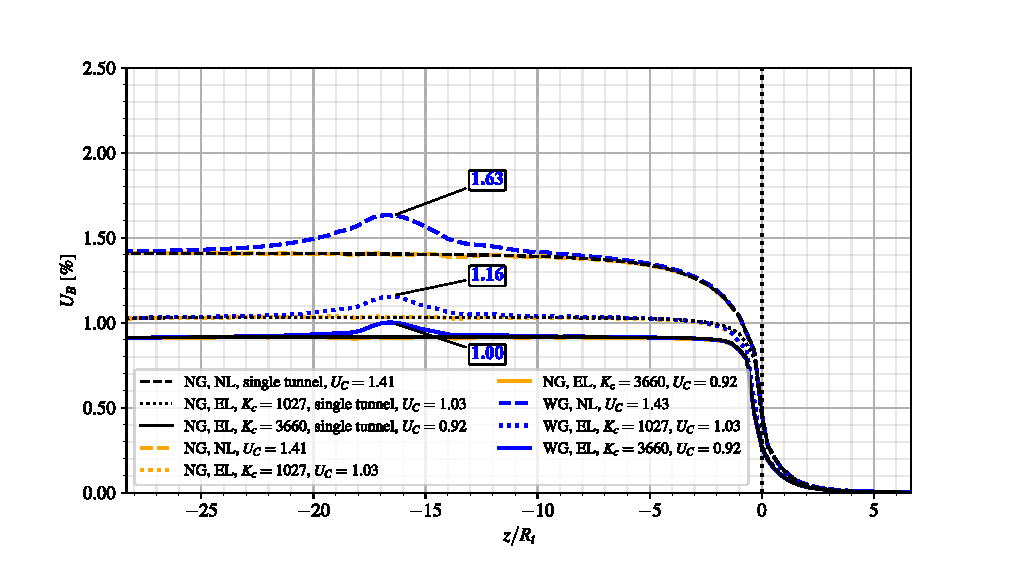
\includegraphics[scale=1]{Figures/Convergence Profiles - EP_d1_16Ri_anotate.pdf}
	\caption{Convergence Profiles - for $d_1 = 16R_t$.}.
	\label{EP_d1_16Ri}
\end{figure}
\FloatBarrier
\begin{figure}[h!]
	\centering
	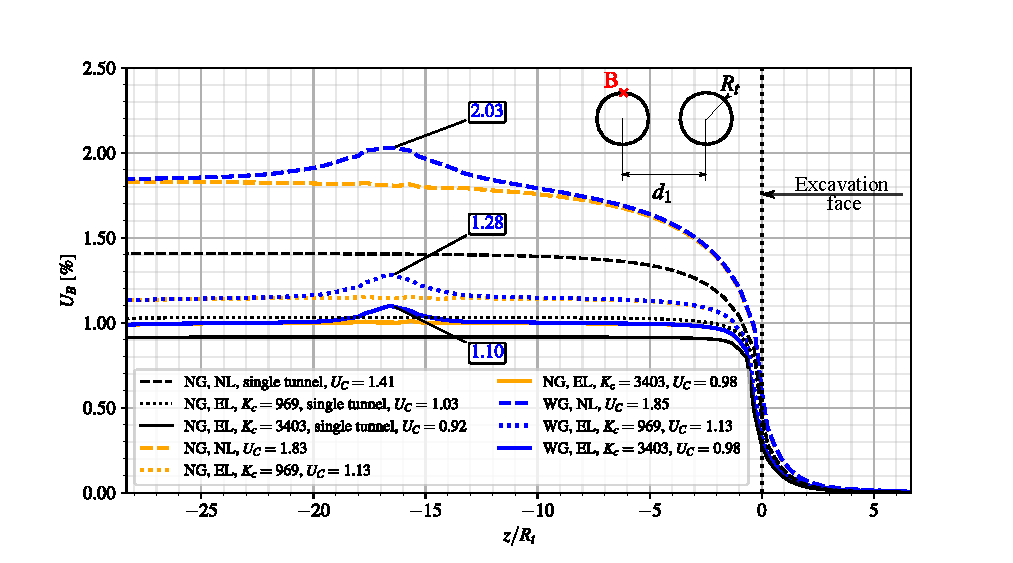
\includegraphics[scale=1]{Figures/Convergence Profiles - EP_d1_4Ri_anotate.pdf}
	\caption{Convergence Profiles - for $d_1 = 4R_t$.}.
	\label{EP_d1_4Ri}
\end{figure}
\FloatBarrier

When comparing results between twin lined tunnels with spacings of $16R_t$ and $4R_t$, differences of 6\% with high stiffness lining (solid yellow and blue lines), 10\% with moderate stiffness lining (dotted yellow and blue lines), and 30\% without lining (dashed yellow and blue lines) are observed. These results show the direct impact of lining stiffness and the distance between twin tunnels on $U_{eq}$ convergence.

When analyzing the convergence $U_{peak}$ at the point where the gallery meets the longitudinal tunnel, there is an increase of 16\% when using an moderate stiffness elastic lining (dotted blue line) compared to a high stiffness lining (solid blue line). However, when analyzing the difference between the $U_{eq}$ and $U_{peak}$, there is a difference of up to 12\% for the high stiffness elastic lining (solid blue line to $4R_t$ and $16R_t$) and up to 13\% for the moderate stiffness elastic lining (dotted blue line to $4R_t$ and $16R_t$) for $d_1=4R_t$.

In both graphs, increased stiffness localizes the gallery's effect on the convergence profile, reducing it from $22.5R_g$ (without lining) to $10.5R_g$ and $7.5R_g$ (with elastic lining) along the longitudinal tunnel. Tunnel proximity had minimal impact on this range.

% --------------------------------------------------------------------------
\section{Conclusions}\label{sec:conclusion}
% --------------------------------------------------------------------------

The analyses show that lining significantly affects the convergence profile of twin tunnels, reducing convergence by up to 35\% and the gallery's localized effect by a third compared to no lining. A less rigid lining (3.5 times less) increased convergence by 12\% and expanded the localized effect by 40\% compared to the most rigid lining. Tunnel interaction becomes significant at 4Rt but minimally impacts in the range of gallery's localized effect.

%-------------------------------------------------------------------------
\vspace{20pt}
\noindent \textbf{Acknowledgements.} The authors are grateful for the financial support provided by CAPES and CNPq.
\vspace{12pt}

%--------------------------------------------------------------------------
\noindent \textbf{Authorship statement.} The authors hereby confirm that they are the sole liable persons responsible for the authorship of this work, and that all material that has been herein included as part of the present paper is either the property (and authorship) of the authors, or has the permission of the owners to be included here. 

\bibliography{bibliography}

\end{document}
% --------------------------------------------------------------------------
